\documentclass{standalone}
\usepackage[T1]{fontenc}
\usepackage[utf8]{inputenc}
\usepackage[english]{babel}
\usepackage{tikz}
\usepackage{times}
\usetikzlibrary{calc,through,backgrounds,positioning,fit}
\usetikzlibrary{shapes,arrows,shadows}
\usetikzlibrary{mindmap}
 
\begin{document}
 
\tikzstyle{place}=[shape=circle, draw, minimum height=10mm]
\tikzstyle{trig}=[shape=circle, draw, dashed, minimum height=10mm]
\tikzstyle{trans}=[shape=rectangle, draw, minimum height=6mm, minimum width=12mm]
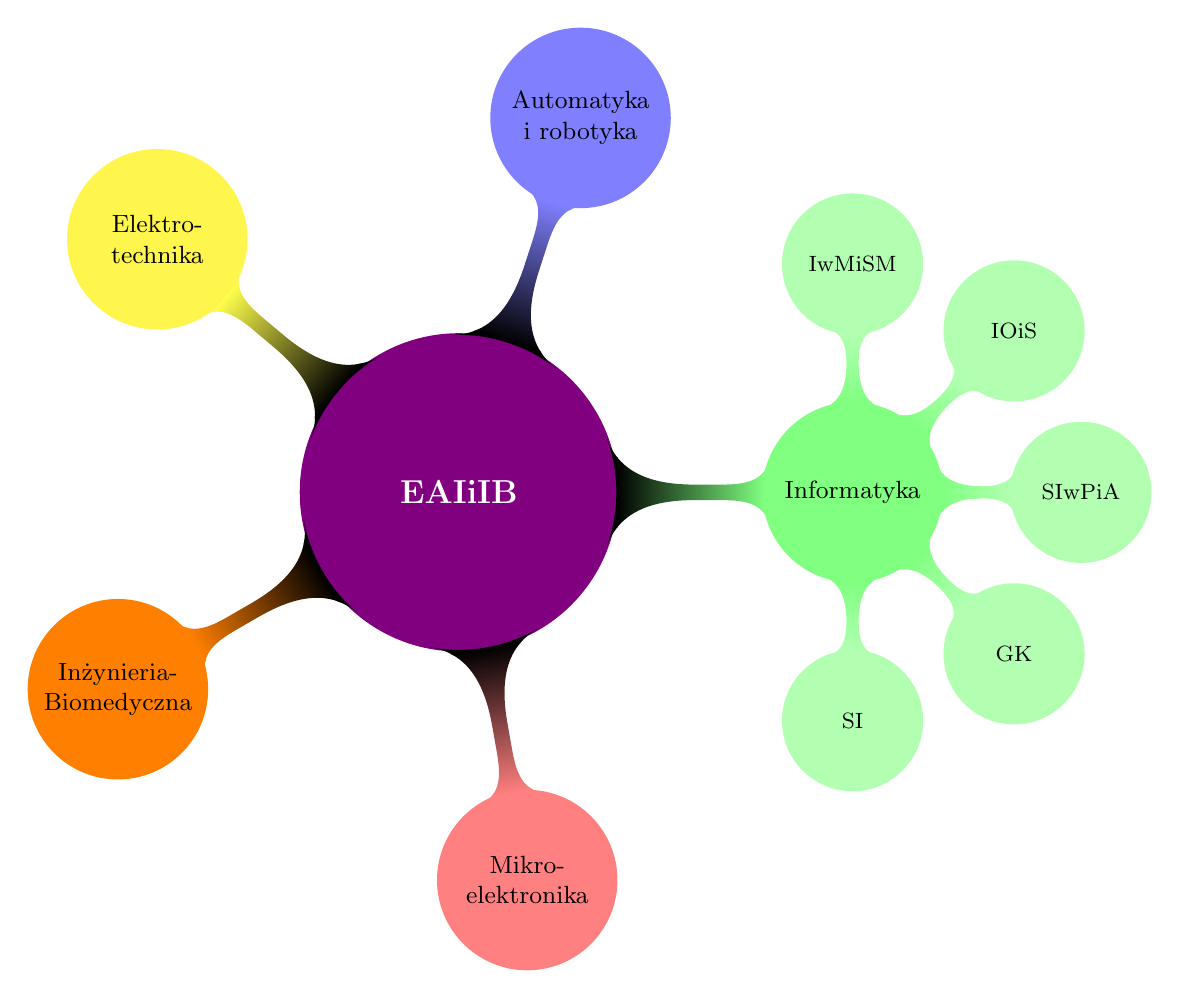
\begin{tikzpicture}[mindmap]
\node [concept,concept color=red!50!blue, text=white] {\bf EAIiIB}
child[grow=-150, concept color=orange!100] {node[concept] {Inżynieria-\\Biomedyczna}}
child[grow=-80, concept color=pink!200] {node[concept] {Mikro-\\elektronika}}
child[grow=140, concept color=yellow!70] {node[concept] {Elektro-\\technika}}
child[grow=72, concept color=blue!50] {node[concept] {Automatyka i robotyka}}
  child[grow=0, concept color=green!50] {node[concept] {Informatyka}
    child[grow=90, concept color=green!30] {node[concept] {IwMiSM}}
	child[grow=45, concept color=green!30] {node[concept]{IOiS}}
	child[grow=0, concept color=green!30] {node[concept]{SIwPiA}}
	child[grow=-45, concept color=green!30] {node[concept]{GK}}
	child[grow=-90, concept color=green!30] {node[concept]{SI}}
    };

\end{tikzpicture} 
\end{document}